%Compila en Texnicenter

% Birthday calendar
% Author: Hakon Malmedal
\documentclass[fontsize=20pt]{scrartcl}

\usepackage[utf8]{inputenc}
\usepackage[T1]{fontenc}
\usepackage{lmodern}
\usepackage[margin=1cm,a4paper,landscape]{geometry}
\pagestyle{empty}
\usepackage{graphicx}
\usepackage{tikz}
\usepackage{pgfplots}  %Axis se define aqui
\usetikzlibrary{calendar,fit}
\usepackage{expl3,xparse}

%% Adapted from http://tex.stackexchange.com/a/10199/4771

\begin{document}

\centering

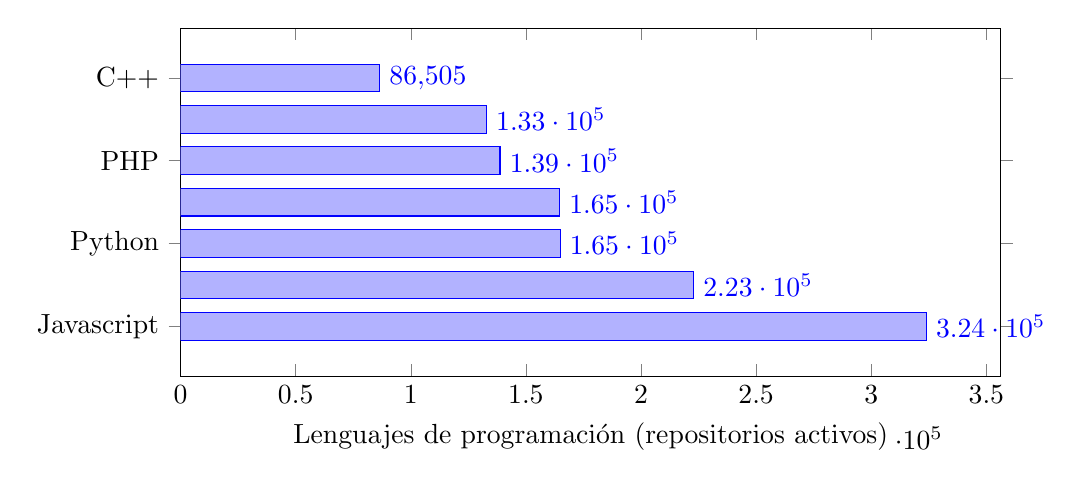
\begin{tikzpicture}[thick]
\begin{axis}[
xbar, xmin=0,
width=12cm, height=6cm, enlarge y limits=0.2,
xlabel={Lenguajes de programación (repositorios activos)},
symbolic y coords={Javascript, Java, Python, CSS, PHP, Ruby, C++},
nodes near coords, nodes near coords align={horizontal},
]
\addplot coordinates {(323928,Javascript) 
(222852,Java)
(164852,Python)
(164585,CSS)
(138771,PHP)
(132848,Ruby)
(86505,C++)};
\end{axis}

\end{tikzpicture}

\end{document}